% LUMC presentation template by J. F. J. Laros.
% Last alteration on 15-10-2009.
%
% The packages texlive-latex-recommended, texlive-latex-base and
%   texlive-latex-extra should be installed.
%

% Alter these four lines for a new presentation.
\providecommand{\me}{Jeroen F. J. Laros}
\providecommand{\myTitle}{Mutalyzer 2.0 $\alpha$}
\providecommand{\myConference}{Work discussion}
\providecommand{\myDate}{Tuesday, 5 January 2010}

% Now go to %%% BEGIN PRESENTATION %%%

\documentclass[a4, portrait]{seminar}

\usepackage{semcolor} % For coloured text.
\usepackage{slidesec} % For section headings.
\usepackage{newcent}  % This is a better font for presentations.
\input{seminar.bug}

\usepackage{graphicx} % For pictures.
\usepackage{fancybox} % For the background picture.

\definecolor{Blue}{rgb}{0.,0.11372,0.37647} % Custom LUMC color

\renewcommand{\labelitemi}{\textcolor{white}{$\bullet$}} % Make the bullets for
\renewcommand{\labelitemii}{\textcolor{white}{--}}       % itemising white.
\renewcommand{\labelitemiii}{\textcolor{white}{$\ast$}}
\renewcommand{\labelitemiv}{\textcolor{white}{$\circ$}}

\newslideframe{TITLE}{ % Template for the title.
  \boxput{
    \rput(0, 0){\includegraphics[angle=90, scale=.485]{bg}}
  }{#1}
}

\newslideframe{PRES}{ % Template for the body.
  \boxput{
    \rput(0, 0){\includegraphics[angle=90, scale=.485]{bg2}}
  }{
    \textcolor{Blue}{
    \rput[l]{90}(8.57, -1.5){\scriptsize{\myConference}} 
    \rput[c]{90}(8.57, 5.35){\scriptsize{\theslide/\pageref{LastPage}}}
    \rput[r]{90}(8.57, 12.2){\scriptsize{\myDate}}
    }
    \white #1
  }
}

\renewcommand{\makeslideheading}[1]{ % Put the slide headings on top.
  \rput[l](0.2, .40){
      \textbf{
        \textcolor{Blue}{#1}
    }
  }
  \newline
}

\pagestyle{empty}

\begin{document}

\slideframe{TITLE} % Use the title template.

\begin{slide}
\setcounter{slide}{0}
\vspace*{1.5cm}
\begin{center}
{\bf\Large{\myTitle}}\\
\vfill
\textcolor{Blue}{
  {\bf
    \small{\me}\\
    \small{Department of Human Genetics}\\
    \small{Center for Human and Clinical Genetics}
  }
}
\vspace{1.1cm}
\end{center}
\end{slide}

\slideframe{PRES} % Use the body template.

%%% BEGIN PRESENTATION %%%

\begin{slide}
\slideheading{Test version}
\begin{center}
We are now testing an $\alpha$-version of Mutalyzer.
\end{center}
\vspace*{1cm}
\begin{itemize}
\item Due to modular design, already used for mapping.
\item Capable of recognising complex variants.
\item Capable of complex checks.
\item Faster.
\item Error handling (demo).
\item Extensive logging.
\end{itemize}
\vfill
\end{slide}

\begin{slide}
\slideheading{Complex variants}
\vspace*{1cm}\\
More than one variations in one allele are recognised and processed, making the
analysis of complex variants possible.
\vspace*{1cm}\\
\texttt{c.[4G>T;18del]} can not be analysed by Mutalyzer 1.0.4, it had to be 
converted to \texttt{c.4\_18delinsTCTAAGTTAAAACT} (highly impractical when 
the raw variants are far apart).
\vfill
\end{slide}

\begin{slide}
\slideheading{Complex checks}
\vspace*{1cm}\\
Deletion of \texttt{gc} from \texttt{tcgcgt} will be corrected as a deletion of
\texttt{cg} (works for all strings).
\vspace*{1cm}\\
Inversion of (partial) palindromes are detected. \texttt{ctgaaacag} will be 
corrected as an inversion of \texttt{aaa} to \texttt{ttt}.
\vfill
\end{slide}

\begin{slide}
\slideheading{Comparing runtime}
\begin{center}
\colorbox{white} {
  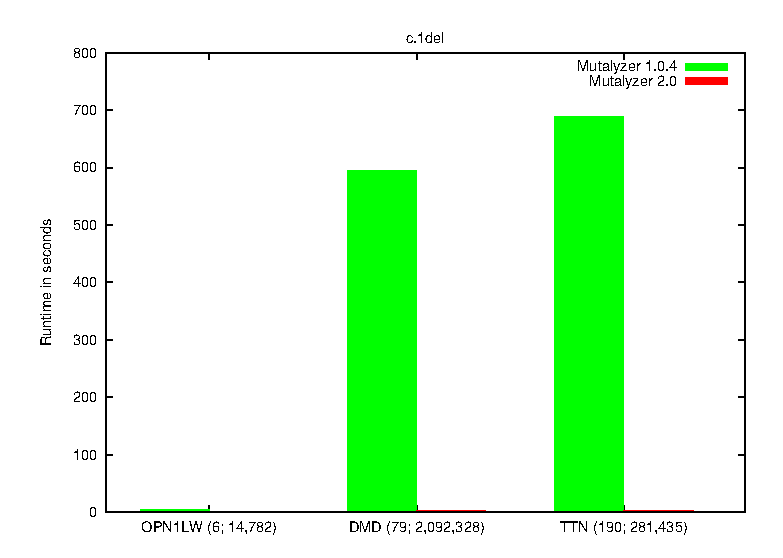
\includegraphics[scale = 0.7]{genes}
}
\end{center}
\vfill
\end{slide}

\begin{slide}
\slideheading{Runtime with increasing complexity}
\begin{center}
\colorbox{white} {
  \includegraphics[scale = 0.7]{allele}
}
\end{center}
\vfill
\end{slide}

\begin{slide}
\slideheading{Logging}
\begin{verbatim}
04-01-2010 14:57:20 Main (Main): Received variant 
                    AB026906.1:c.54_55del
04-01-2010 14:57:20 Main (Main): Finished processing 
                    variant AB026906.1:c.54_55del
04-01-2010 16:32:31 Main (Main): Received variant 
                    AB026906.1:c.54_55delf
04-01-2010 16:32:31 Main (Parser): Error: Expected 
                    end of text (at char 21), 
                    (line:1, col:22)
04-01-2010 16:32:31 Main (Main): Finished processing 
                    variant AB026906.1:c.54_55delf
\end{verbatim}
\vfill
\end{slide}

\begin{slide}
\slideheading{Prospects}
\vspace*{1cm}\\
\begin{itemize}
\item Overhead is $\pm 2.5s$.
\item Processing time is $\pm 0.1s$.
\item Batches can be converted to a multi-allele description: e.g. 
      \texttt{c.[1del];[4\_5dup]}.
\item Provided that more than one variant is given for one reference sequence, 
      processing time for a batch job is negligible.
\end{itemize}
\vfill
\end{slide}

\begin{slide}
\slideheading{Future plans}
\vspace*{1cm}\\
\begin{itemize}
\item Compile the corrections to a new variant description.
\item Implement protein descriptions.
\item Better visualisation.
\item Automatically generate a description by comparing two sequences.
\end{itemize}
\vfill
\end{slide}

\begin{slide}
\rput(11.4,0.6){
\includegraphics[scale=0.1]{Gen2Phen}}
\slideheading{Questions?}
\vfill
\label{LastPage}
\end{slide}

\end{document}
